
GIM alebo Glucose-Insulin Model softvér nám dáva schopnosť simulovať chovanie sa jedinca a jeho sekréciu inzulínu.\cite{2007}

V poslednej dobe bol navrhnutý nový model simulácie jedla, ktorý umožnil meranie rôznych tokov, glukózy a inzulínu, vyskitujúcich sa počas jedla. V skutočnosti je systém, veľmi zložitý a iba dostupnosť tokov glukózy a inzulínu, ich plazmatických koncentrácií, nám umožní minimalizovať štruktúrne neistoty pri modelovaní rôznych procesov. Model pozostáva z 12 nelineárnych diferenciálnych rovníc, 18 algebraitických rovníc a 35 parametrov.\cite{2007}

Užívateľsky príjemný simulačný softvér tohto modelu by bol veľkou pomocou, najmä pre vyšetrovateľov bez konkrétnych odborných znalostí v oblasti modelovania.Softvér GIM, implementovaný v MATLAB verzii 7.0.1, ktorý umožňuje simulovať normálne aj patologické stavy, napr. Diabetes typu 2 a inzulín s otvorenou a uzavretou slučkou infúzie pri cukrovke 1. typu. Softvér sa nepokúša riešiť patofyziologické otázky.\cite{2007}

\subsection{MATLAB Version}

GIM softvér je založený na MATLAB-e. Ako je možné vidieť nižšie na uvedených obrázkoch(\ref{okna}), nie to to vôbec jednoduché na pochopenie. Tým pádom bežný pacient tenot softvér nevie využiť. Ak vás zujíma bližšie fungovanie tohto softvéru, prečítajte si o ňom v tejto správe zo sympózia, kde bol prvýkrát uvedený do používania \cite{2007}.

\begin{figure}[H]
\centering
 \begin{subfigure}[b]{0.475\linewidth}
   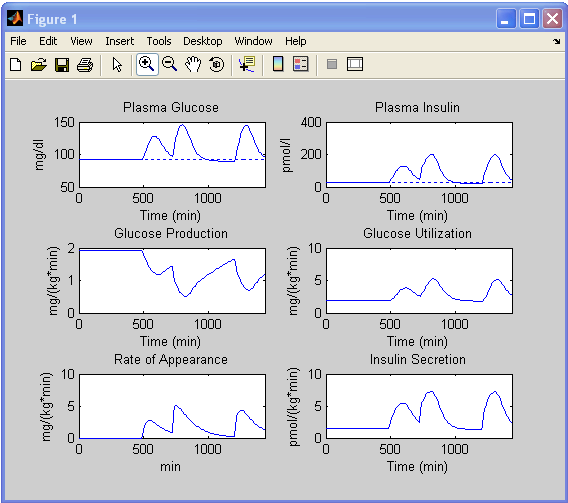
\includegraphics[width=\linewidth]{ob-3.PNG}
   \caption{Vystup}
 \end{subfigure}
 \begin{subfigure}[b]{0.475\linewidth}
   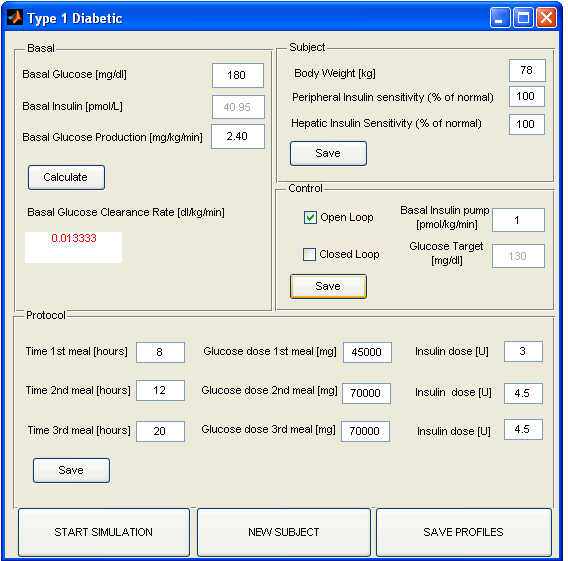
\includegraphics[width=\linewidth]{ob-4.PNG}
   \caption{vstup}
 \end{subfigure}
\caption{Dialogove okna v GIM \cite{2007}}
\label{okna}
\end{figure}

\paragraph{Grafické vyjadrenie informácií v informatike}
Viete v informatike, keď sa pripravuje nejaký softvér treba dbať aj na konečného užívateľa. Dobrým príkladom môže byť GIM. Jeho prostredie väčšine laikom povie akurát tak nič. Treba mať presne zadefinované, kto bude daný softvér používať. V prípade GIM simulátora sú to lekári a laboratórny pracovníci. Ak si vezmeme iný, voľne dostupný softvér pre diabetikov, je omnoho ústretovejší a prehľadnejší pre laikov, bežných ľudí.